\subsection{Variation explained by principal components}
\label{sec:variationExplainedPCA}

The most visual way of explaining the variation as a function of principal components, is an cumulative plot of the squared principal components (diagonal elements of the $\Sigma$ matrix after executing \texttt{svd} as explained in section 3.3 in the course notes\cite{coursenotes}):

\begin{figure}[H]
 \centering
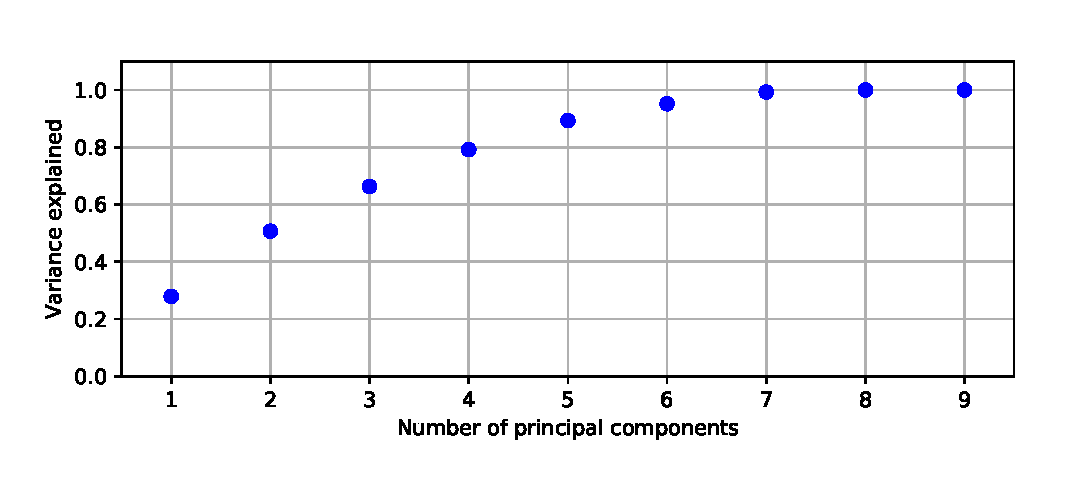
\includegraphics[width=0.9\linewidth]{fig/RhoAkk.eps}
\caption{Accumulated explained variance of data as function of principal components.}
\label{fig:rhoakk}
\end{figure}

In fig \ref{fig:rhoakk} we see, that two principal components only account for $\sim$50\% of the variation/information in the dataset. In order to get close to 90\% at least 5 principal components are needed. This might be expected from section \ref{sec:CorrMat} when inspecting the weak correlations between most of the attributes. 